331.\begin{figure}[ht!]
\center{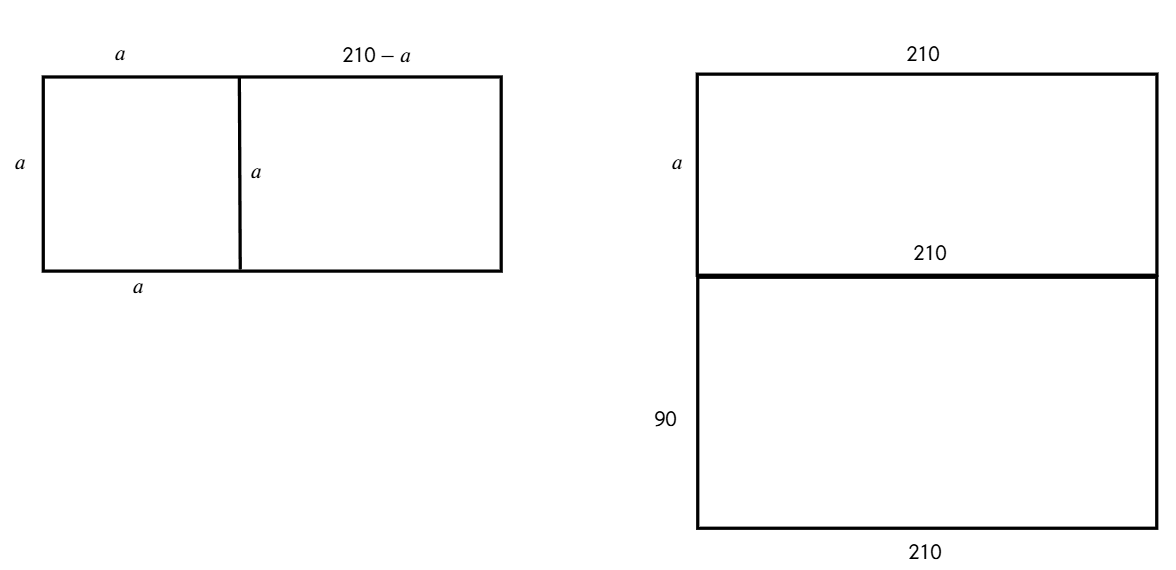
\includegraphics[scale=0.35]{kv5.png}}
\end{figure}\\
Если у прямоугольника периметр равен 420 см, то его стороны в сумме дают $420:2=210$см, то есть они равны $a$ и $210-a.$ Так как после отрезания получился квадрат, всего его стороны равны $a$ (см. левый рисунок). Тогда одна из сторон исходного прямоугольника была равна $a+210-a=210$см. Поэтому у прикладываемого прямоугольника вторая сторона равна $600:2-210=90$см (см. правый рисунок). Так как после прикладывания получился квадрат, должно выполняться равенство $a+90=210,\ a=210-90=120$см. Таким образом, исходный прямоугольник имел размеры $120\text{ см}\times210\text{ см}.$\\
